\chapter{Analysis}\label{ch:Analysis}

In the first step of the waterfall model, requirement and object analysis is carried out.

\section{Defining use cases}
Based on the description given, actors and use cases are identified and then clearly defined.

\subsection{Actors}
Based on the project description provided, the only actor that we have found would be the user who is running the simulation. At first we had considered the database to be an actor of the system but later discovered that it would not be that appropriate to have the database as an actor to the system.

\subsection{Use cases}
Next, we have defined the various use cases that we want the user to be able to do, which will be described in the following sections.

\subsubsection{Add node}
When the user wants to add the node, they would need to specify the type of node added. The node added could be either a IoT Node or a network gateway.

\subsubsection{Start Simulation}
When the user wants to start the simulation, they would need to provide the following information:
\begin{itemize}
  \item Number of nodes in the network
  \item Size of the 2D grid where the nodes will be placed
  \item Option of verbose output
\end{itemize}

\subsubsection{See simulation statistics}
When the user wants to see simulation statistics, the system would need to check if any simulation has occurred previously. If there is no prior simulation, then the system would display an error. Otherwise, the system would display the simulation statistics such as throughput, delay, and packet loss.

\subsection{Use case diagram}
Based on the factors mentioned above, a use case diagram was developed. The use case diagram can be seen below.

\subsection{FURPS}

The FURPS were utilized to better define the system's requirements. The system's overall summary was also created using this technique. This approach also aided in providing a fresh and more enlightening perspective on the issue and the requirements.

\subsubsection{Functionality: what should the system do?}
\begin{itemize}
  \item The system should be able to place the nodes in a grid and transmit packets from one node to the gateway.

        %\item The system would need to place different type of nodes in the network

  \item The system would need to run the simulation for a fixed amount of time


\end{itemize}

\subsubsection{Usability: what kind of UI is needed?}
\begin{itemize}
  \item A screen would be required to display the simulation statistics
  \item A device should receive user input eg.keyboard
\end{itemize}

\subsubsection{Reliability: what is the tolerance of the system to failures?}
\begin{itemize}
  \item The system should be able to check if the simulation has been run before displaying simulation statistics
\end{itemize}

\subsubsection{Performance: which response times, accuracy, availability, resource usage should the system have?}

\begin{itemize}
  \item The GUI needs to be run on a simple computer
  \item The simulation statistics needs to be stored in a server
\end{itemize}

\subsubsection{Sustainability: what adaptations may be needed?}
\begin{itemize}
  \item The system need to give the user the ability to change the simulation conditions after a run has been completed
\end{itemize}

\section{Domain model}
To aid the group in identifying the various objects involved in the problem, a domain model was developed. Firstly, the identified actor, which is the user, is represented as a GUI in the model. This also constitutes the front end of the system. Regarding the back end of the system, we would need one object to simulate the network and another one to generate/store the simulation statistics. Ultimately, we would need an object for the devices themselves and one for the overall network. Here it might also be a viable option to differentiate between a node object and a gateway object that then both can inherit attributes and methods from the device object when making the class diagram. Then, in order to control everything and tie the simulation to gather, it would make sense to incorporate a simulation object that handles the simulation itself.

\begin{figure}[H]
  \centering
  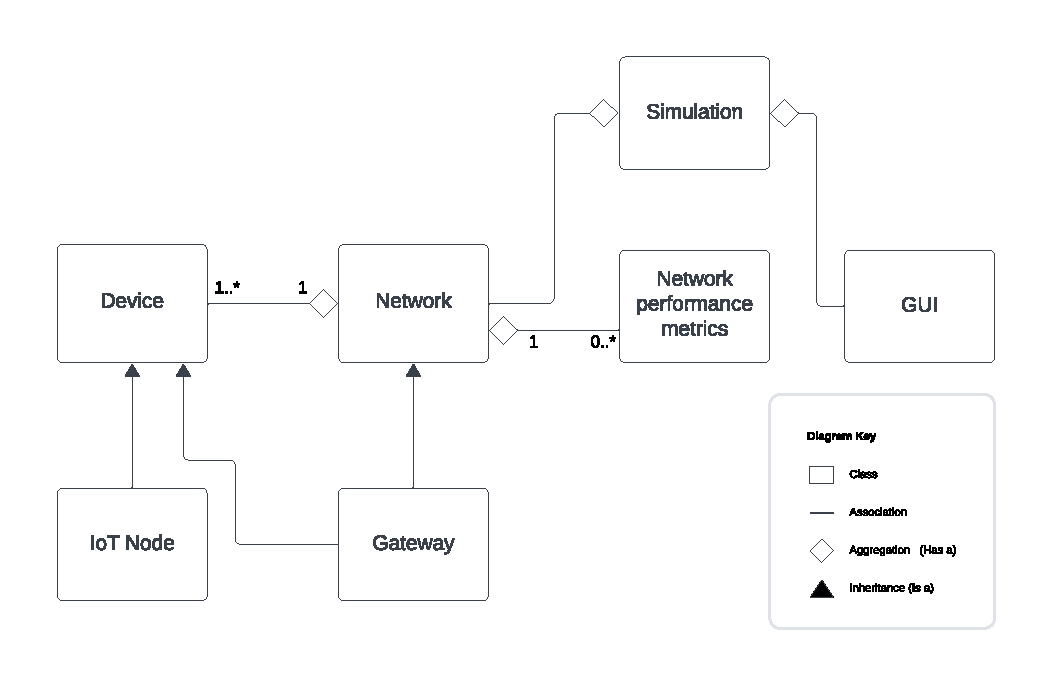
\includegraphics[width=\textwidth]{Domain_model.pdf}
  \caption{Diagram of the domain model.}
  \label{fig:Domain_model}
\end{figure}

\section{Class diagram}
The entirety of the class diagram can be seen in \autoref{fig:Class_diagram}. The parts that were not implemented have their text colored red. This also implies that the class diagram is made in accordance to how the implementation has been done, where it then has been changed whenever something has been changed in the program itself.

\begin{figure}[H]
  \centering
  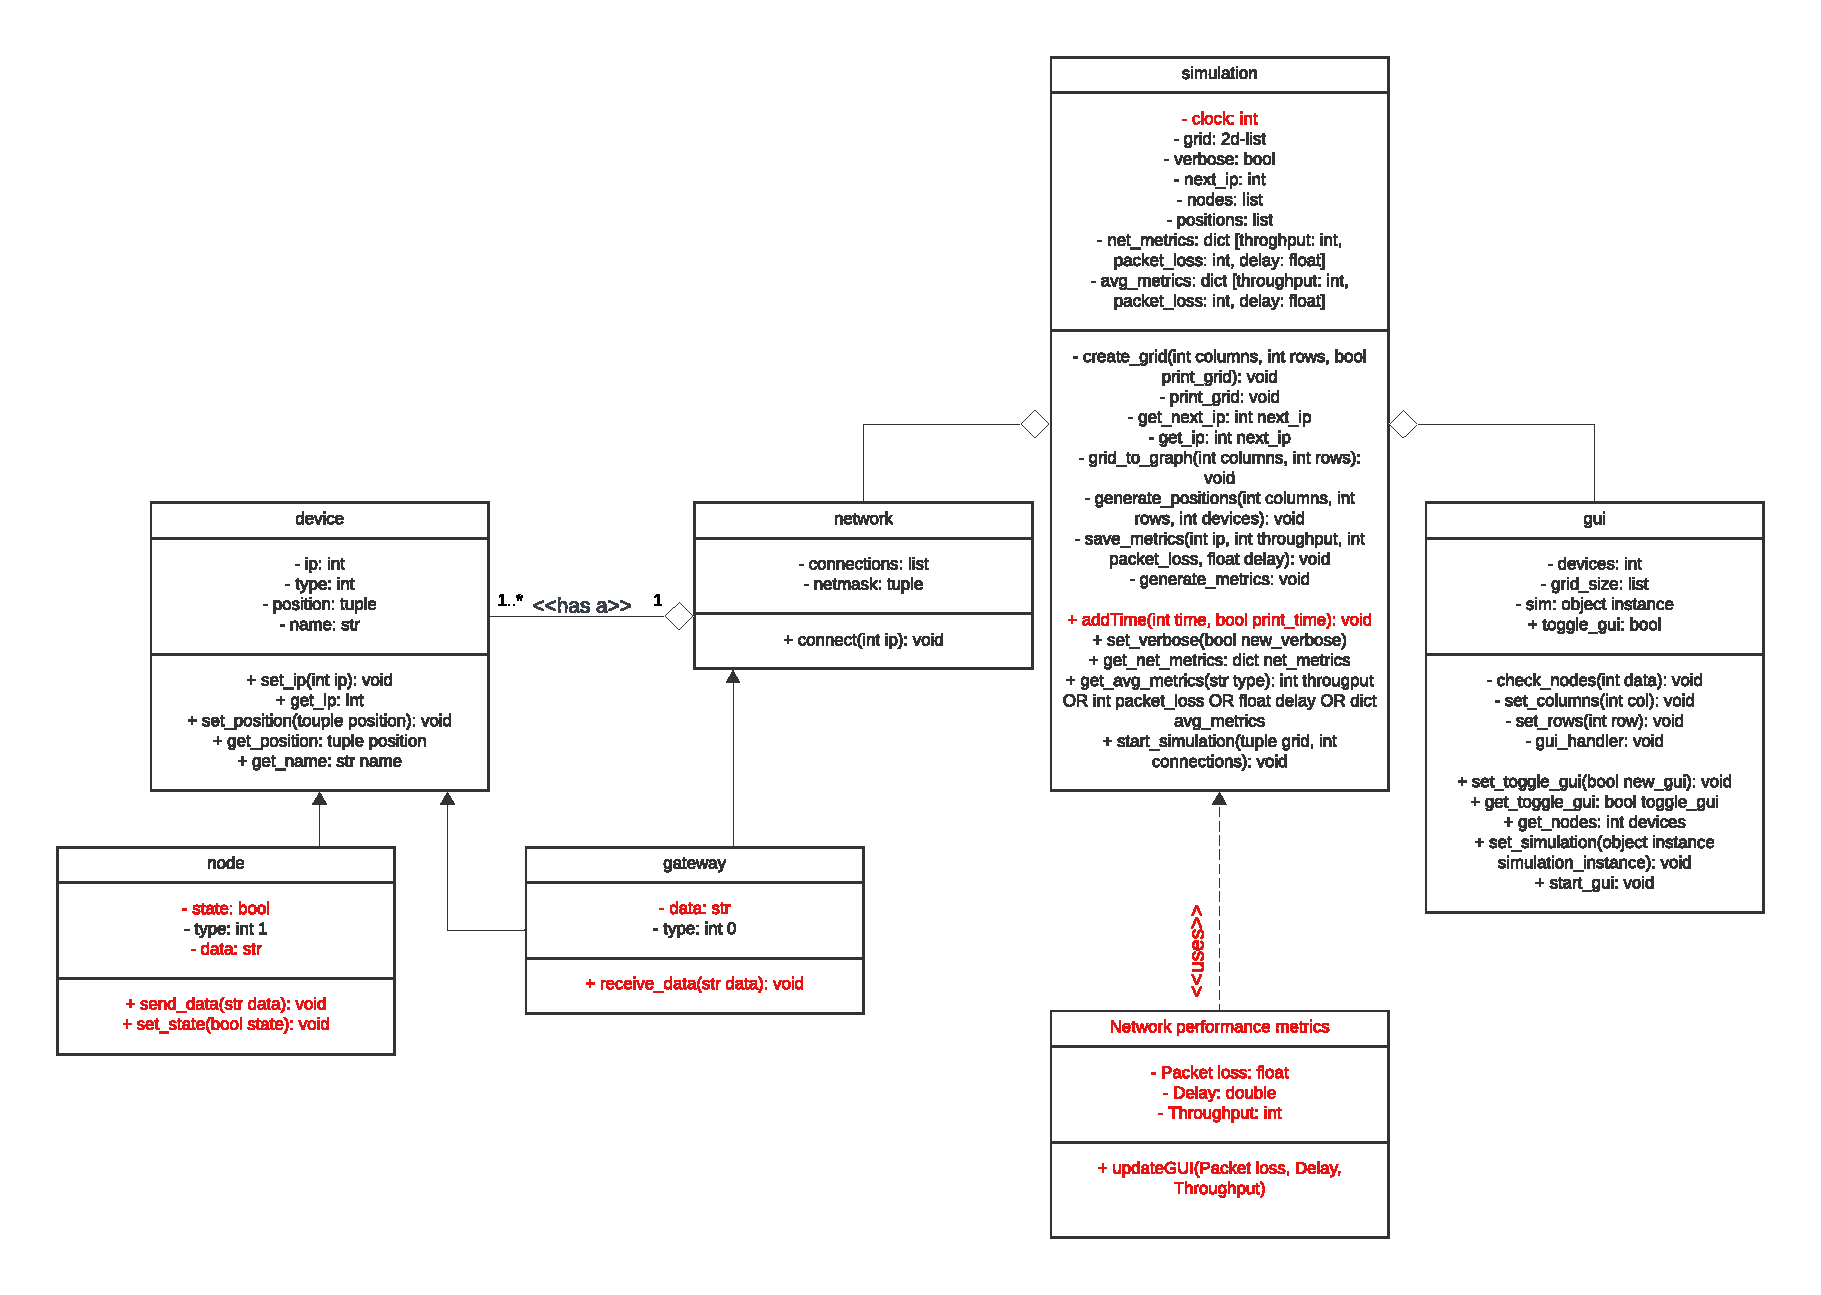
\includegraphics[width=\textwidth]{UML class diagram.pdf}
  \caption{Diagram of the classes.}
  \label{fig:Class_diagram}
\end{figure}

\subsection{GUI} It needs to be possible for the rest of the system to function without a GUI, which will also make it easier to test whether the rest of the program functions as expected. Since this is also the object that the user will interact with, it should also be somewhat easy to use. In order to start the GUI itself a \code{start\_gui} method is needed that can then be called from the main program file. Since PyWebIO is used to program the GUI, the built-in method, called \code{start\_server} can then be called to open a port on the transport layer, which then in turn can be used to access the GUI from any other computer with network access to the computer executing the program. When \code{start\_server} is called, another method can be passed along as an argument, which is then how the GUI is controlled for the remaining time. This method is called \code{gui\_handler}, and it decides which elements of the GUI is shown as well as receiving input from the user and calling other methods of the \code{gui} object.

\subsection{Network}
This class is missing a lot of the attributes and methods that it should have managed instead of the \code{simulation} object. As it is currently implemented, the \code{network} object only stores a list of the IP-addresses that are currently reserved by the gateway or one of the nodes.\bigbreak

\noindent Conventionally, on local networks, only the digits after the last period in the IP-addresses differentiate the different devices in the network. Therefore, it is only necessary to store the differentiating part of the IP-addresses. This means that the attribute \code{connections} must be able to contain a list of integers from 1 to some maximum number of devices in the network. Additionally the simulation ended up being in charge of creating connections between the gateway and the nodes, even though this should definitively have been a method of the \code{device} object that \code{node} and \code{gateway} would then have been able to use to reserve an IP-address in the \code{connections} attribute of the \code{network} object.\newline

\noindent To put it differently, the \code{network} object should have more coupling to make it more clear that it is in charge of the network functionality, that its name is implying. Even though the \code{simulation} is necessary, it should have been possible to view all of the network methods and attributes in the \code{network} object instead of needing to also view the \code{simulation} object.

\subsection{Device}


\subsubsection{Node}


\subsubsection{Gateway}


\subsection{Simulation}
The simulation is the object that takes over right after getting called by the \code{gui} object. It is then in charge of controlling the simulation. The first thing that happens is then that the \code{start\_simulation} method is accessed by the \code{gui\_handler} method which passes on the input from the user, namely the attributes \code{devices}, and \code{grid\_size}. By called its own method \code{simulation} can then use \code{create\_grid} to create an empty grid of the size specified by the previously mentioned attributes.\bigbreak

\noindent Right after creating the empty grid, the \code{gateway} object is instantiated, it gets the IP-address 1 by using calling the \code{get\_next\_ip} method, and its position is then set to the middle of the empty grid and stored both in the \code{gateway} object as well as the \code{simulation} object. Even though it was implemented this way it should only have been stored in the \code{gateway} object.





























